\chapter{Введение}

{\bf Актуальность.} На рубеже нулевых и десятых годов XXI века, параллельно идущие процессы удешевления как средств, так и услуг мобильного доступа в сеть Интернет, а также удешевления и миниатюризации средств спутниковой навигации привели к появлению принципиально нового вида онлайн-услуг --- служб, основанных на местоположении (location-based service, LBS)\cite{ruwikilbs}. Одним из таких сервисов является удалённое наблюдение за местонахождением транспортных средств, с помощью установленных на них автономных <<маяков>>, различными способами определяющих собственное местонахождение и передающих данные о нём через мобильный интернет. Владельцы личных автомобилей преимущественно используют подобные средства в следящих противоугонных системах\cite{enwikivetrasy}, но эти средства применимы и в городском транспортном хозяйстве. Помимо непосредственно городских властей, в чьи интересы входит наблюдение за транспортными потоками для задач городского планирования, пресечения злоупотребления служебным положением со стороны недобросовестных водителей и прочих глобальных целей, подобные данные могут быть интересны и простым пассажирам. В связи с трудностью прогнозирования транспортной обстановки, реальный график движения наземного общественного транспорта в часы пик может существенным образом отличаться от расписания. Наблюдение же реальной динамики движения позволило бы создать систему, делающую динамически изменяющиеся прогнозы фактического времени прибытия транспорта и предполагаемого времени в пути, о результатах которого уведомляющую пассажиров через такие каналы как электронные табло на остановках и в самих транспортных средствах, через беспроводную связь подключённые к серверу системы, web-сервис, доступный через стационарные или планшетные компьютеры, приложение для смартфонов (см. рис. \ref{fig:yakazan}), SMS или USSD сервис для любого типа мобильных телефонов и другие. Подобные системы уже начинают внедрять по всему миру\cite{itsrapidbus}\cite{spbtrans}\cite{novosib}\cite{yakazan}, однако по-прежнему сравнительно высокая стоимость приёмников GPS и ГЛОНАСС тормозит процесс внедрения. С другой стороны, существуют сервисы позиционирования мобильных телефонов, использующие для своей работы только информацию о сигналах от базовых станций сотовой сети, но их проблемой является недостаточная точность позиционирования. При этом, на общественном транспорте используются те же системы, что и на личном, хотя между ними есть огромная разница: общественный транспорт движется по заранее известным и неизменным маршрутам, что фактически позволяет свести задачу его позиционирования от двухмерного случая к одномерному. Но эта технологическая ниша оказалась фактически незанятой.

\begin{figure}[h]
	\center{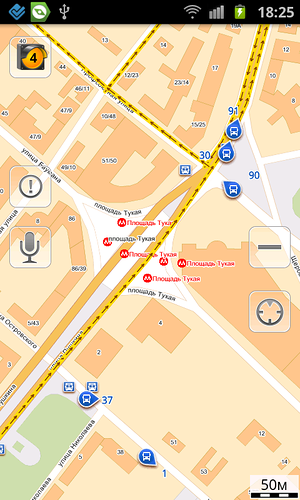
\includegraphics[width=0.5\linewidth]{yakazan.png}}
	\caption{Приложение от Яндекс, в реальном времени показывающее автобусы Казани. Изображение из блога Яндекса\cite{yakazan}}
	\label{fig:yakazan}
\end{figure}

{\bf Целью} данной работы является проверка предположения о возможности существенного повышения точности позиционирования транспортных средств, по сравнению с существующими универсальными системами, при условии заранее известного маршрута движения, а также удешевления подобной системы, по сравнению со случаем использования спутниковой навигации. Для достижения этой цели требуется создать и протестировать прототип подобной системы позиционирования, который, в случае успеха, в дальнейшем может быть доработан до промышленного образца, внедрён и коммерциализирован, однако эти цели уже выходят за рамки данной работы.

{\bf Задачи}, которые требуется решить на пути к данной цели, таковы:

\begin{itemize}
	\item
		Формулировка одномерной задачи позиционирования на местности;
	\item
		Анализ принципов работы существующих систем позиционирования и поиск в них избыточности относительно одномерной задачи позиционирования;
	\item
		Создание математического метода, устраняющего указанную избыточность в пользу большей точности;
	\item
		Проектирование архитектуры системы с учётом разработанного метода и реализация её прототипа:
	\item
		Тестирование созданного прототипа.
\end{itemize}

{\bf Публикации.} Помимо данной пояснительной записки, результаты данной работы также были дважды представлены на разных стадиях на конференции студентов, аспирантов и молодых специалистов МИЭМ (см. <<\nameref{chap:publications}>> на стр. \pageref{chap:publications}). Данная работа также выиграла конкурс грантов <<Участник Молодёжного Научно-Инновационного Конкурса>> в марте 2011 года\cite{umnikwinners}.
